\chapter{Τεχνολογίες}

Με τις γλώσσες προγραμματισμού έχουμε απεριόριστες δυνατότητες, με μόνο περιορισμό τη φαντασία μας.
Ο προγραμματισμός είναι μια διαδικασία που υφίσταται 
εδώ και πάρα πολλά χρόνια, και έχει εξελιχθεί ραγδαία. Η εξέλιξη αυτή οδήγησε στην ανάπτυξη τεχνολογιών, εργαλείων και βιβλιοθηκών ανοιχτού κώδικα που μας επιτρέπουν να υλοποιούμε με ευκολία λειτουργίες στα προγράμματα μας που διαφορετικά θα ήταν ιδιαιτέρως χρονοβόρες.
Αυτά τα εργαλεία έχουν σχεδιαστεί έτσι ώστε να είναι προσαρμόσιμα σε κάθε περίπτωση και για κάθε χρήση, μέσω μερικών απλών ρυθμίσεων.

Η χρήση τέτοιων εργαλείων επιτρέπει σε έναν προγραμματιστή να επικεντρωθεί στην ουσία του προγράμματος παρά στις υλοποιήσεις της υποδομής και της ασφάλειας. Τέτοια εργαλεία έχουν χρησιμοποιηθεί για την ανάπτυξη αυτής της πτυχιακής. Παρακάτω αναφέρονται μερικά από τα πιο σημαντικά εργαλεία που χρησιμοποιήθηκαν.

\section{JHipster}

\begin{figure}[h]
  \centering
  
\includegraphics[]{Chapters/3 - Technologies/Images/jhipster-logo.png}
  \caption{Λογότυπο JHipster}
  \label{fig:jhipster-logo}
\end{figure}

Το JHipster είναι ένα εργαλείο αυτόματης παραγωγής κώδικα. Στόχος του είναι η αυτόματη δημιουργία αρχείων κώδικα τα οποία επαναλαμβάνονται για κάθε εφαρμογή του είδους.

Για παράδειγμα, για την δημιουργία μιας υπηρεσίας API στην Java, χρησιμοποιώντας μια βάση δεδομένων SQL, κατά προτίμηση πρέπει αρχικά να επιλεγεί ένα Web Framework, για να διευκολύνει την διαχείριση και την ανάπτυξη του προγράμματος. Αφού επιλεγεί αυτό το Framework, πρέπει να ρυθμιστεί ανάλογα για να καλύψει τις ανάγκες της εφαρμογής. Στην συγκεκριμένη περίπτωση πρέπει να ρυθμιστεί να στέλνει δεδομένα τύπου JSON ή XML αφού ο στόχος είναι η δημιουργία μιας υπηρεσίας API. Πρέπει επίσης να ρυθμιστεί η σύνδεση με την βάση δεδομένων, πρέπει να ρυθμιστεί πως θα εμφανίζονται οι ημερομηνίες στις απαντήσεις... κ.ο.κ. 

Το JHipster δημιουργεί όλα αυτά τα αρχεία και τις ρυθμίσεις δίνοντας την επιλογή περαιτέρω ρύθμισης και με αυτόν τον τρόπο εξοικονομεί χρόνο από την ρύθμιση της υποδομής και επιτρέπει άμεση εστίαση στην υλοποίηση της εφαρμογής γνωρίζοντας ότι υπάρχει μια ισχυρή υποδομή που έχει δημιουργηθεί από το JHipster με την επιλογή της επιπρόσθετων ρυθμίσεων για την βελτιστοποίηση της λειτουργίας της εφαρμογής.

Εκτός από τις ρυθμίσεις επιτρέπει τη δήλωση του Μοντέλου της εφαρμογής στην JDL DSL του, και μπορεί να δημιουργήσει τα ανάλογα Entities, Services Και Controllers και στο Frontend και στο Backend.

Η πτυχιακή αυτή αρχικά δημιουργήθηκε με το JHipster χρησιμοποιώντας το Spring Framework για το backend και την React Library για το Frontend. Επιπρόσθετα προσέθεσε ρυθμίσεις και για αρκετά άλλες τεχνολογίες που χρησιμοποιήθηκαν.


\section{Backend}
\subsection{Spring Framework}

\begin{figure}[h]
  \centering
  
\includegraphics[]{Chapters/3 - Technologies/Images/spring-logo-9146a4d3298760c2e7e49595184e1975.png}
  \caption{Λογότυπο Spring Framework}
  \label{fig:spring-logo}
\end{figure}

Το Spring Framework είναι ένα Framework και IoC Container που στοχεύει στην εύκολη ανάπτυξη, διαχείριση και συντήρηση μιας εφαρμογής μεγάλου μεγέθους. Έχει σχεδιαστεί για να χρησιμοποιείται σε οποιουδήποτε είδους εφαρμογής αλλά προσφέρει επεκτάσεις και πακέτα για την ανάπτυξη Web Υπηρεσιών πάνω στην πλατφόρμα Java EE ~\citep{wiki:spring}

Το Spring Framework είναι η καρδία του Backend της πτυχιακής καθώς πάνω σε αυτήν έχει δομηθεί και όλος ο κώδικας.

\subsection{ElasticSearch}

\begin{figure}[h]
  \centering
  
\includegraphics[width=85mm]{Chapters/3 - Technologies/Images/elastic-search-logo-color-horizontal.png}
  \caption{Λογότυπο Spring Framework}
  \label{fig:elasticsearch-logo}
\end{figure}
Η ElasticSearch, είναι μια μηχανή αναζήτησης πραγματικού χρόνου και ανάλυσης δεδομένων. Βασίζεται στο lucene της Apache, μια υψηλών επιδόσεων με αρκετά χαρακτηριστικά βιβλιοθήκη για μηχανές αναζήτησης. ~\citep{wiki:elastic}

Χρησιμοποιείται για την αναζήτηση Ηθοποιών, Εταιριών \& Χωρών Παραγωγής και Ειδών Ταινιών, από το Frontend με μεσολαβητή το Backend.
\section{Frontend}
\subsection{React Library}
\begin{figure}[h]
  \centering
  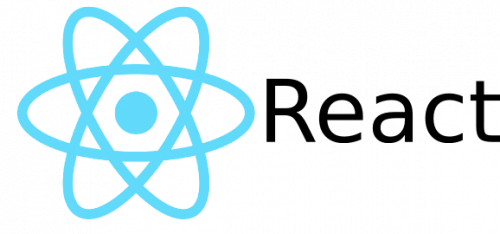
\includegraphics[width=75mm]{Chapters/3 - Technologies/Images/react-logo_1.png}
  \caption{Λογότυπο React}
  \label{fig:react-logo}
\end{figure}
Η React είναι μια βιβλιοθήκη γραμμένη σε JavaScript με σκοπό την εύκολη δημιουργία SPA Σελίδων, και δημιουργήθηκε από την Facebook.
Χαρακτηρίζεται βιβλιοθήκη και όχι Framework καθώς είναι μινιμαλιστική και διαθέτει πολύ απλές λειτουργίες και βασίζεται σε άλλα OpenSource πακέτα για τις πιο σύνθετες λειτουργίες όπως Routing, State Management κ.α.

Το Frontend της πτυχιακής χρησιμοποιεί σαν κύρια τεχνολογία την React σε συνδυασμό με το Redux.
\subsection{Redux}

\begin{figure}[h]
  \centering
  
\includegraphics[width=75mm]{Chapters/3 - Technologies/Images/redux-logo.png}
  \caption{Λογότυπο Redux}
  \label{fig:redux-logo}
\end{figure}

Το Redux είναι ένα προβλέψιμο state container για εφαρμογές JavaScript. Θεωρείται προβλέψιμο διότι το State (κατάσταση της εφαρμογής) είναι αμετάβλητο και σε κάθε πρόθεση αλλαγής γίνεται αντικατάσταση. Με αυτόν τον τρόπο καθίσταται δυνατή η αλλαγή του State της εφαρμογής οπουδήποτε μέσα στο ιστορικό (undo,redo). Επίσης διευκολύνει το debugging καθώς δεν υπάρχει mutability και επομένως η χρονική στιγμή και οι παράγοντες κάθε αλλαγής είναι ορατοί ανά πάσα στιγμή/συνεχώς.

Το Redux δεν σχεδιάστηκε για την React, αλλά μεγάλο μέγεθος εφαρμογών γραμμένων σε React το χρησιμοποιούν λόγω
των μεγάλων δυνατοτήτων και της απλότητας του. Οι δημιουργοί του Redux δημιούργησαν επίσης ένα επίσημο πακέτο για την εύκολη επικοινωνία της React με το Redux, με όνομα react-redux. 

Το react-redux χρησιμοποιήθηκε στο Frontend της Πτυχιακής,
μαζί με κάποιες ακόμα επεκτάσεις του για την λήψη των δεδομένων από το Backend καθώς και για το Caching. Χρησιμοποιήθηκε επίσης και για την δρομολόγηση των αποτελεσμάτων που θα εμφανίζονται.